\section{Reference Wire Scanner measurements}\label{sec:sps_transverse_beam_profiles}
\subsection{Example beam profiles}
Figures~\ref{fig:WS_example_profiles_H_2022} and~\ref{fig:WS_example_profiles_V_2022} show two example horizontal and vertical beam profile as obtained from the SPS.BWS.51637.H and SPS.BWS.41677.V instruments respectively during the experiment with CC1 in SPS in 2022. The data points from the IN (OUT) scan are shown with a blue (orange) color. 

The measured data points (light blue) are fitted with a four-parameter gaussian (orange) following the procedure discussed in Section~\ref{subsec:sps_ws} to obtain the beam size. Thereafter, the emittance values and their uncertainties are computed from Eqs.~\eqref{eq:emittance_from_WS} and~\eqref{eq:emittance_from_WS_uncertainty} respectively. The results of the fit are also shown in the plots. It is evident that the calculated uncertainties are two orders of magnitude smaller than the corresponding emittance values themselves. This is the case for all acquisitions. However, not all the profiles are displayed in this thesis for practical reasons.

\begin{figure}[htp]
    \centering
    \begin{subfigure}{.45\textwidth}
        \centering
        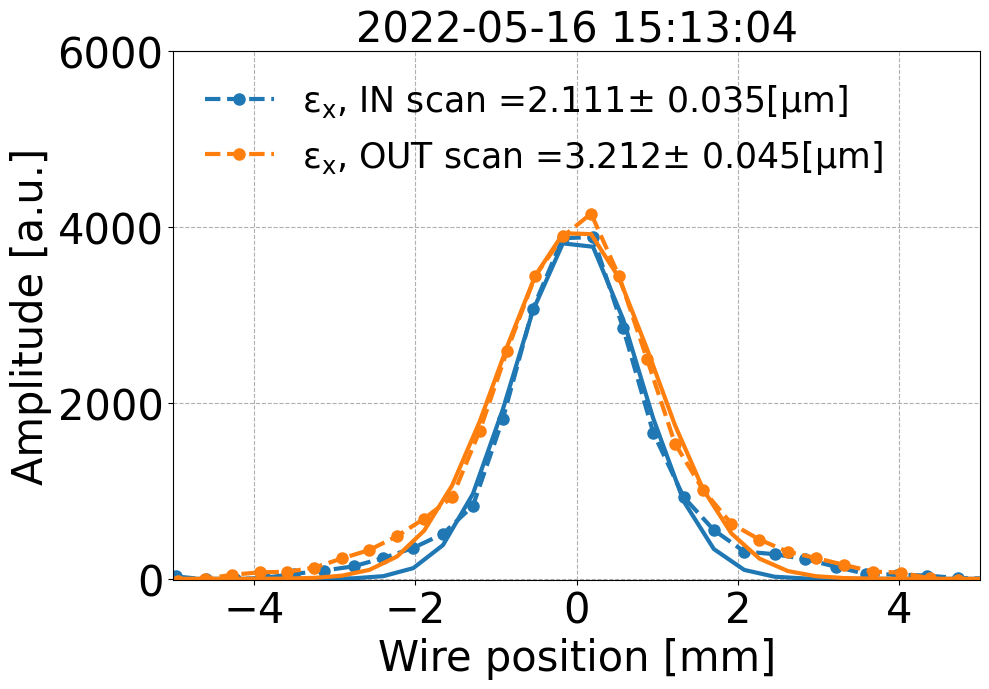
\includegraphics[width=.95\linewidth]{images/app_c/SPS.BWS.51637.H_IN_OUT_ 15_13_04.png}  
        \caption{Horizontal beam profile.}
        \label{fig:WS_example_profiles_H_2022}
    \end{subfigure}
    \begin{subfigure}{.45\textwidth}
        \centering
        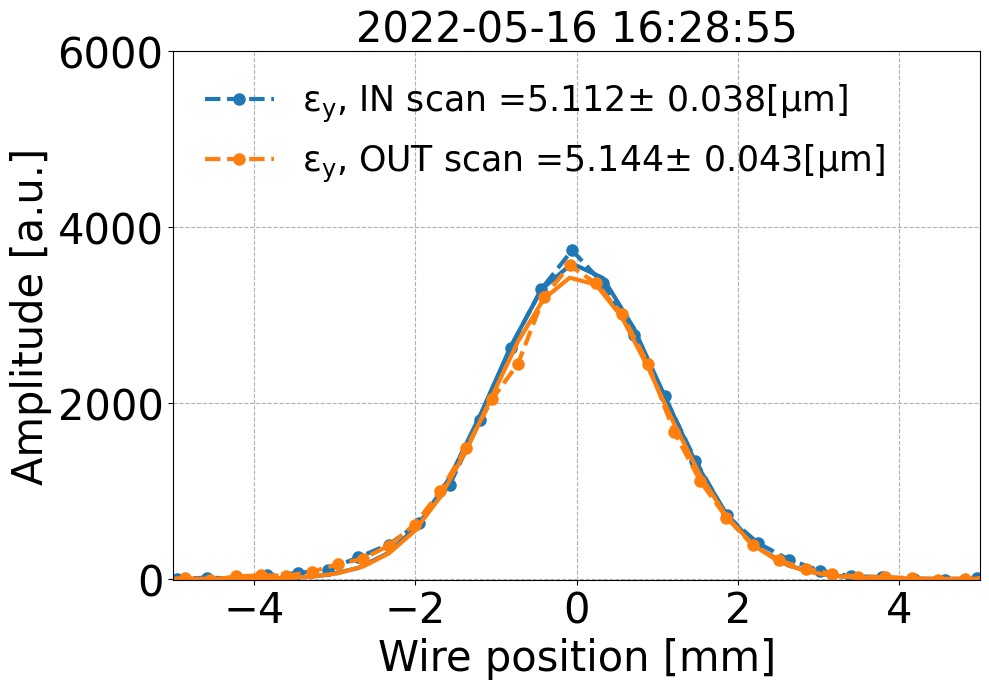
\includegraphics[width=.95\linewidth]{images/app_c/41678.V_IN_OUT_ 16_28_55.png}  
        \caption{Vertical beam profile.}
        \label{fig:WS_example_profiles_V_2022}
    \end{subfigure}
    \caption{Transverse beam profiles as obtained from SPS.BWS.51637.H during the CC experiment in the SPS in 2022. The data points from the IN (OUT) scan are shown with blue (orange) color.}
    \label{fig:WS_example_profiles_H_V_2022}
 \end{figure}
 

%\begin{figure}[!h]
 %   \centering         
 %   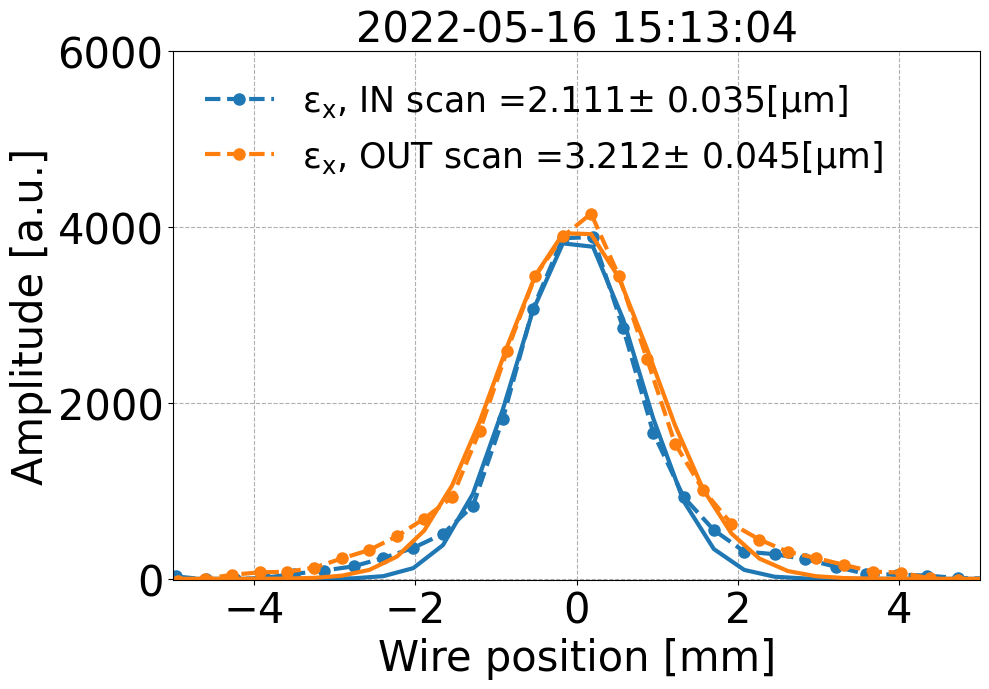
\includegraphics[width=0.6\textwidth]{images/app_c/SPS.BWS.51637.H_IN_OUT_ 15_13_04.png}
 %       \caption{Horizontal beam profile as obtained from SPS.BWS.51637.H during the CC experiment in the SPS in 2022. The data points from the IN (OUT) scan are shown with blue (orange) color. }
%        \label{fig:WS_example_profiles_H_2022}
 %\end{figure}

 %\begin{figure}[!h]
 %   \centering         
 %   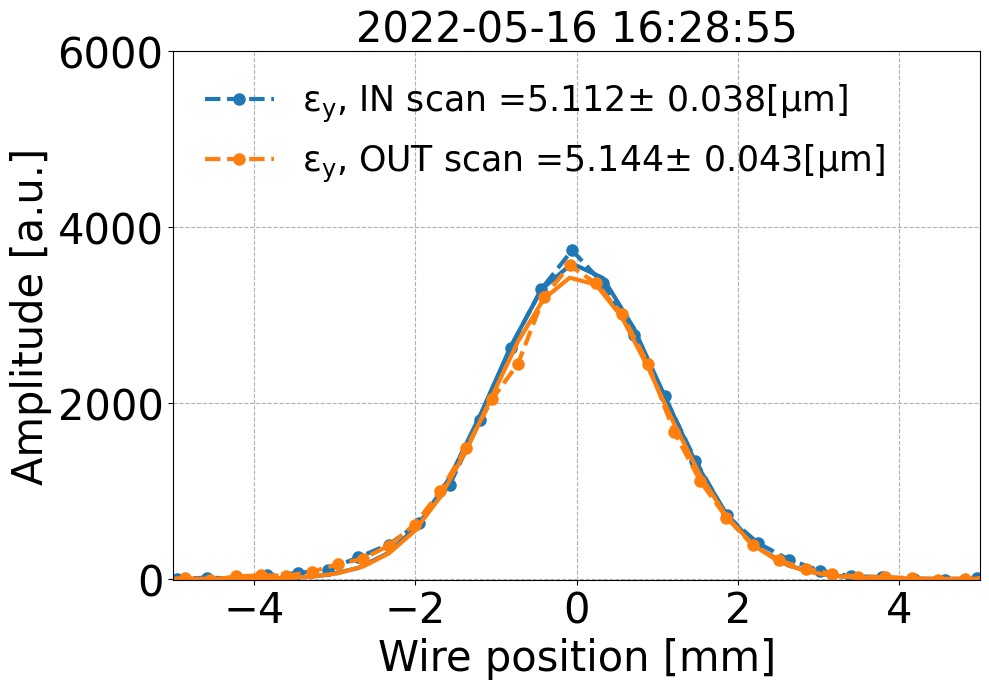
\includegraphics[width=0.6\textwidth]{images/app_c/41678.V_IN_OUT_ 16_28_55.png}
 %       \caption{Vertical beam profile as obtained from SPS.BWS.51637.H during the CC experiment in the SPS in 2022. The data points from the IN (OUT) scan are shown with blue (orange) color. }
 %       \label{fig:WS_example_profiles_V_2022}
 %\end{figure}

 \subsection{Emittance values from IN and OUT scan}\label{subsec:ex_emit_growth_in_vs_out}
 Figure~\ref{fig:WS_IN_vs_OUT_2022} shows the transverse emittance evolution acquired with  SPS.BWS.51637.H and SPS.BWS.41677.V for horizontal and vertical planes respectively during the experiment with CC noise on May 16, 2022. The emittance values acquired during the IN scan are shown on the left while the ones acquired during the OUT scan are shown on the right. 

It can be seen that the emittance values obtained from the OUT scan appear to be more fluctuated than the values from the IN scan. In this particular example, this is enhanced in the horizontal plane (blue). It is also clearly visible for the acquisitions during the first half of the coast.

% Path to data:/eos/user/n/natriant/2022/SPS_MDs_2022/cc_md_16May2022/roundA_online_analysis_ws/for_thesis/coast8
% Relevant slides: https://docs.google.com/presentation/d/1QIaQNfqVWaI8cHGGgb5eeS7c_jdUMuxLqD_poHrOtH0/edit#slide=id.g148272a84c8_2_0
 \begin{figure}[htp]
    \centering
    \begin{subfigure}{.45\textwidth}
        \centering
        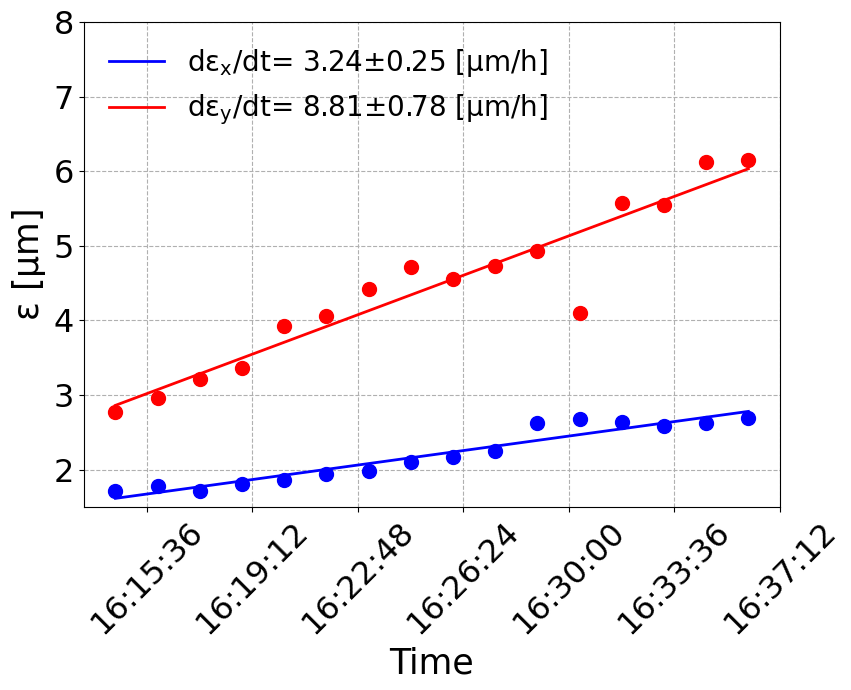
\includegraphics[width=.95\linewidth]{images/app_c/ws_coast8_set1.png}  
        \caption{Emittance evolution from IN scan.}
        \label{fig:WS_example_profiles_H_2022}
    \end{subfigure}
    \begin{subfigure}{.45\textwidth}
        \centering
        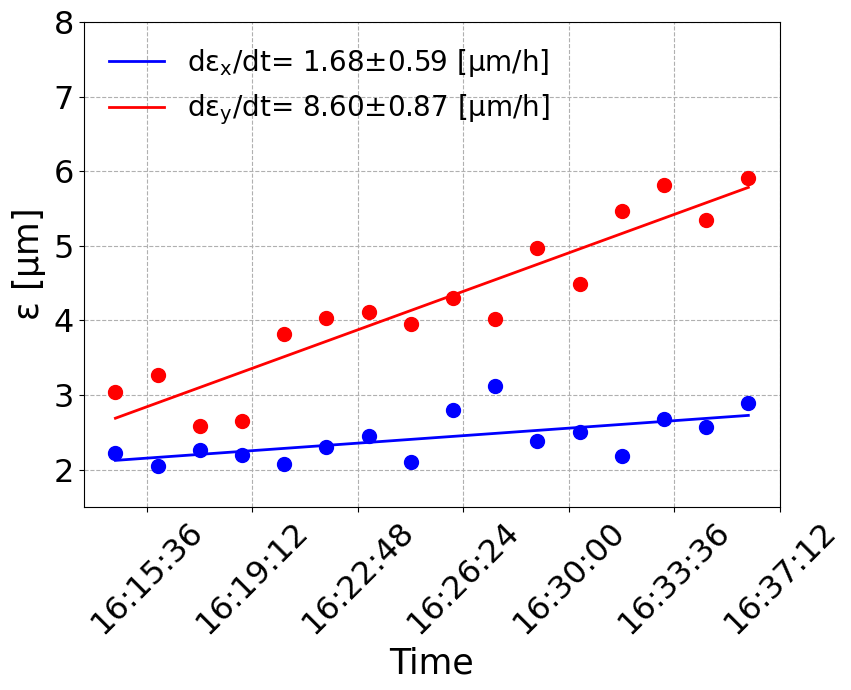
\includegraphics[width=.95\linewidth]{images/app_c/ws_coast8_set2.png}  
        \caption{Emittance evolution from OUT scan.}
        \label{fig:WS_example_profiles_V_2022}
    \end{subfigure}
    \caption{Transverse beam profiles as obtained from SPS.BWS.51637.H during the CC experiment in the SPS in 2022. The data points from the IN (OUT) scan are shown with blue (orange) color.}
    \label{fig:WS_IN_vs_OUT_2022}
 \end{figure}
